% MICCAI submission — Springer LNCS format. 双盲:提交版匿名,正文 8 页(不含参考文献)。
% 数字来源:paper/tables/numbers.json(由 analysis/paper_figs.py 生成)与 docs/vlm_backbone.md;
% 已撤回的表述(AUC 0.85、宽松硬过滤 0.803、随机森林 0.812、"头部区域排序"、"门控与骨架无关")不得出现。
\documentclass[runningheads]{llncs}

\usepackage[utf8]{inputenc}
\usepackage[T1]{fontenc}
\usepackage{graphicx}
\usepackage{booktabs}
\usepackage{amsmath,amssymb}
\usepackage{xcolor}
\usepackage[hidelinks]{hyperref}

\newcommand{\todo}[1]{\textcolor{red}{[TODO: #1]}}
\newcommand{\asd}{ASD}
\tolerance=1500 \emergencystretch=1.2em

\begin{document}

\title{Where Clinicians Look Tells Us What to Measure:\\
Attention-Defined Gait Measurements and Evidence-Gated Fusion for Adult Spinal Deformity}
\titlerunning{Where Clinicians Look Tells Us What to Measure}

% ==== 提交时保持匿名 ====
\author{Anonymous Submission}
\authorrunning{Anonymous Submission}
\institute{Paper ID \todo{ID}}

\maketitle

\begin{abstract}
Clinician region annotations are usually injected into gait models as attention supervision.
On lateral-view gait videos of adult spinal deformity (\asd) patients we show that this buys
interpretability but not accuracy: a region-grounded 3D CNN reproduces clinician attention
four times better than Grad-CAM while patient-level balanced accuracy stays at $0.64$--$0.66$,
a video transformer does no better, and four skeleton models are at chance. We instead let the
annotations decide \emph{what to measure}: the regions clinicians mark define five sagittal
quantities from 3D keypoints, and a logistic regression on these five numbers reaches $0.72$
(AUC $0.79$; 67 patients, 10 random splits)---above every end-to-end model, above five random
measurements (98th--100th percentile) and four quantities at unmarked regions ($0.66$), and
equal to the best data-driven selection over 1,272 candidates. We then fuse the five numbers
with the video model by an evidence-strength rule---trust the measurements when they deviate
from the population norm, defer to video otherwise---which raises $0.75$ to $0.79$ ($0.82$
with the grounded model) where a nested global weight gives $0.75$, and passes permutation,
region-specificity, backbone and leave-one-out controls. The deviation signal is carried by
head posture, uninformative alone but decisive given trunk inclination.
\keywords{Clinical priors \and Gait analysis \and Interpretability \and Adult spinal deformity.}
\end{abstract}

\section{Introduction}

Adult spinal deformity (\asd) alters walking in ways clinicians recognise at a glance from a
lateral view: the trunk inclines forward and the pelvis, hips and knees compensate to keep
the head over the feet~\cite{glassman2005sagittal,schwab2012srs}. Video-based assessment
needs no markers, and it is natural to ask experts \emph{where they look} and to feed that
attention into a deep model as a grounding loss on its saliency or as a modality aligned to
the video~\cite{koh2020cbm,radford2021clip}---treating the annotation as something the
network should \emph{learn from}.

We report a controlled study on 79 patients (1,889 gait videos) annotated by two clinicians
that reaches a different conclusion about what the annotation is for. (i) Used as
supervision, it buys a verifiable attention map---our region-grounded 3D CNN aligns with
clinician attention at $0.53$ against $0.14$ for Grad-CAM---but no accuracy: every
end-to-end video model, from a Kinetics-pretrained 3D CNN to a video transformer, stays at
$0.53$--$0.66$ patient-level balanced accuracy, and four skeleton models are at chance.
(ii) The annotation is a poor training signal: six distinct region combinations, 45.7\%
inter-clinician agreement. (iii) Yet it is highly informative about \emph{what to measure}:
five sagittal quantities at the marked regions, from 3D keypoints and a logistic regression,
reach $0.72$ (AUC $0.79$), and no data-driven selection over 1,272 candidates beats them.

We therefore recast clinician attention from a training signal into a \emph{measurement
prior} (Fig.~\ref{fig:pipeline}): the marked regions decide which quantities are measured, a
readable linear model decides from them, and the annotation is never used at inference. The
grounded video model and the five numbers err on different patients, and we combine them
without a post-hoc weight: an \emph{evidence-strength gate} measures how far a patient's
five quantities deviate from the population norm; unremarkable measurements carry no
evidence and the video decides, otherwise the measurements decide. Learned inside the
cross-validation, the rule lifts $0.75$ to $0.79$ ($0.82$ with the grounded model), and its
signal is carried by head posture relative to the trunk---which is why, we suggest,
clinicians mark the head.

Our contributions are: (1) a matched comparison of one annotation used as supervision versus
as a measurement prior, under one protocol; (2) five clinician-defined measurements that
beat all end-to-end models, with random-measurement, unmarked-region and candidate-bank
controls showing that the value lies in the selection; (3) an evidence-strength gate
validated by permutation, region-specificity, backbone and leave-one-out controls; (4) a
full account of what did not work, in the supplement.

\section{Related Work}

Concept bottlenecks~\cite{koh2020cbm} and attention supervision make a network's
representation match expert concepts or regions; the payoff is a checkable explanation and
the usual finding, as here, is unchanged accuracy. Post-hoc saliency such as
Grad-CAM~\cite{selvaraju2017gradcam} is the common alternative; we measure that it does not
recover clinician attention here. Kinetics-pretrained video
networks~\cite{kay2017kinetics,feichtenhofer2019slowfast,bertasius2021timesformer} and
skeleton graph networks~\cite{yan2018stgcn,chen2021ctrgcn} are the standard end-to-end
choices, whereas clinical gait analysis relies on a few named kinematic quantities.
Selecting measurements by $\ell_1$ regression~\cite{tibshirani1996lasso,guyon2003feature}
and combining classifiers at the probability level~\cite{kittler1998combining} are
classical; we test whether the expert boundary improves selection and gate the fusion by
evidence strength rather than a learned mixture, in the spirit of interpretable-by-design
models~\cite{rudin2019stop}.

\section{Method}
\label{sec:method}

\begin{figure}[t]
\centering
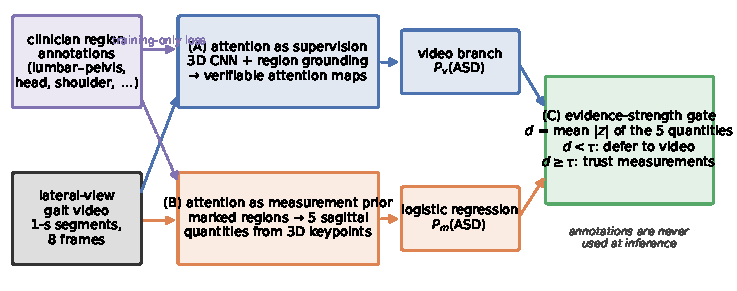
\includegraphics[width=0.86\linewidth]{figs/fig1_pipeline.pdf}
\caption{Two uses of one clinician annotation. (A) As supervision: a region-grounded 3D CNN
with verifiable attention (Sec.~\ref{sec:sup}). (B) As a measurement prior: the marked
regions define five sagittal quantities from 3D keypoints, classified by logistic regression
(Sec.~\ref{sec:prior}). (C) An evidence-strength gate decides per patient whether the
measurements carry enough evidence to decide (Sec.~\ref{sec:gate}).}
\label{fig:pipeline}
\end{figure}

\paragraph{Data and annotation.} Lateral-view walking videos of 79 patients (54 \asd, 25
non-\asd; the latter pools dropped-head syndrome and lumbar stenosis / hip osteoarthritis),
1,889 videos cut into 1-s segments of 8 frames (14,048 segments). Two clinicians marked, per
patient, the regions they attend to from five candidates; at least one clinician marked
lumbar--pelvis for 72\% of patients, head for 47\%, shoulder for 23\%, wrist for 3\% and foot
for 1\%. Only six combinations occur and the clinicians agree on 45.7\% of region decisions.
2D keypoints come from YOLOv8-pose~\cite{TODO_yolov8pose}; camera-frame 3D keypoints from
SAM-3D-Body~\cite{TODO_sam3dbody} exist for 67 patients, the primary cohort.

\subsection{Attention as supervision (contrast)}
\label{sec:sup}

A Kinetics-pretrained slow\_r50 token grid is queried by $R{=}5$ learned concept vectors,
one per region, by cross-attention; each yields an attention map $A_r$ and a pooled feature.
A presence head predicts whether region $r$ is marked and the classifier consumes the
presence-weighted concept features with a global feature. Training minimises
$\mathcal{L}_{\mathrm{cls}} + \lambda_p\mathcal{L}_{\mathrm{presence}} +
\lambda_g\mathcal{L}_{\mathrm{ground}}$: a soft cross-entropy against the two-annotator
targets $\{0,\tfrac12,1\}$ and a KL divergence between $A_r$ and a Gaussian rendering of
the region on the skeleton, weighted by the soft presence. Inference uses video only.
Alignment is $\sum_n A(n)\hat M(n)$, $\hat M=M/\max M$; a uniform map scores $0.068$.

\subsection{Attention as a measurement prior}
\label{sec:prior}

The annotation statistics single out three regions, for which we take the textbook sagittal
readings, computed per segment from its 8 frames: \emph{trunk lean}, the angle of the
shoulder-midpoint--hip-midpoint line to the vertical (forward positive); \emph{shoulder
offset}, the anterior offset of the shoulder midpoint from the hip midpoint over trunk
length; \emph{head forward}, the angle of the ear-midpoint--shoulder-midpoint line to the
vertical; \emph{maximum hip flexion}, $180^\circ$ minus the smallest shoulder--hip--knee
angle; and \emph{hip range}, the within-segment range of that angle. A patient is the mean
of each quantity over segments; the five values are standardised and classified by a
class-balanced logistic regression ($C{=}1$). Nothing is tuned on the outcome. To test
whether the selection matters we also build a \emph{bank} of 1,272 candidates (pairwise
landmark inclinations, offsets and distances, and chain angles, as segment means, extremes
and ranges), each labelled by the regions it touches, and classify it by segment-level
$\ell_1$ logistic regression ($C$ by an inner split) with the candidates restricted to the
clinician regions, to their complement, or unrestricted, and by random forests and gradient
boosting on all candidates.

\subsection{Evidence-strength gating}
\label{sec:gate}

Let $P_v$ and $P_m$ be the patient-level \asd\ probabilities of the video and five-number
models, and $d$ the patient's mean absolute $z$-score of the five quantities with respect to
the training patients. The fused probability is $P=(1-w)P_v+wP_m$ with
$w=w_{\mathrm{lo}}$ if $d<\tau$ and $w=w_{\mathrm{hi}}$ otherwise, $\tau=Q_q(d_{\mathrm{train}})$,
where $(q,w_{\mathrm{lo}},w_{\mathrm{hi}})$ are chosen on the training patients of each outer
fold from a small grid ($q\in\{0.2,\ldots,0.5\}$, $w_{\mathrm{lo}}\in\{0,0.25,0.5\}$,
$w_{\mathrm{hi}}\in\{0.75,1\}$) by balanced accuracy; the test fold only applies the rule:
unremarkable measurements carry no evidence, so the video decides. Under the same nested
protocol we compare a fixed $w{=}0.5$, a nested global $w$, stacking (logistic regression on
the two logits) and a sigmoid gate $w=\sigma(\theta^\top u)$ on six reliability features
(video confidence and segment disagreement, number of segments, measurement confidence,
fraction of segments without 3D, and $d$), fitted by class-balanced likelihood with an
inner-selected $\ell_2$ penalty.

\section{Experiments}

\paragraph{Protocol.}
\label{sec:protocol}
All splits are patient-disjoint. Video and skeleton models use one nested five-fold split
(train/validation/test $\approx$ 60/20/20; validation selects the checkpoint), 50 epochs,
three seeds and identical optimisation (Adam, $10^{-4}$, weight decay $10^{-3}$, bf16); only
the video transformer, unstable at that rate ($0.571$), is reported at $2\times10^{-5}$.
Measurement models have no training randomness, so we re-draw the five-fold partition ten
times and report mean $\pm$ s.d.\ (the fixed split is $0.03$--$0.05$ optimistic for some
variants). Fusion is bound to the fixed split and reported over three video branches (3D
CNN, grounded, grounded without the grounding loss) $\times$ three seeds $=$ nine groups.
Twelve patients have no 3D keypoints and would be median-filled, so primary numbers use the
67 complete patients (46 \asd\ / 21 non-\asd); the 79-patient version is in the supplement.
The metric is patient-level balanced accuracy (segment probabilities averaged per patient;
chance $0.5$) with AUC, bootstrap intervals and exact McNemar tests~\cite{mcnemar1947note}.

\subsection{Main result}

\begin{table}[t]
\centering
\caption{Patient-level balanced accuracy and AUC, 67 patients. Video/skeleton rows: fixed
split, 50 epochs $\times$ 3 seeds. Measurement rows: 10 random partitions. Fusion: fixed
split $\times$ 3 seeds $\times$ 3 video branches.}
\label{tab:main}
\setlength{\tabcolsep}{4pt}
\resizebox{\linewidth}{!}{\begin{tabular}{llcc}
\toprule
Method & Input & Balanced acc. & AUC \\
\midrule
3D CNN (slow\_r50, K400) & video & 0.644±0.045 & 0.670±0.021 \\
TimeSformer-B (K400, 8 frames) & video & 0.637±0.055 & 0.716±0.020 \\
2D CNN (frame average) & video & 0.572±0.044 & 0.591±0.071 \\
CNN--LSTM & video & 0.529±0.015 & 0.582±0.074 \\
CLIP alignment (needs annotation at test) & video+annot. & 0.589±0.030 & 0.600±0.027 \\
3D CNN + region grounding (Sec.~3.1) & video & 0.663±0.030 & 0.694±0.091 \\
ST-GCN, 2D skeleton & skeleton & 0.513±0.010 & 0.563±0.019 \\
ST-GCN, 3D skeleton & skeleton & 0.538±0.026 & 0.557±0.038 \\
CTR-GCN, 2D skeleton & skeleton & 0.491±0.029 & 0.521±0.066 \\
CTR-GCN, 3D skeleton & skeleton & 0.528±0.065 & 0.553±0.078 \\
Random forest, 1,272 measurements & 3D meas. & 0.732±0.019 & 0.736±0.019 \\
Gradient boosting, 1,272 measurements & 3D meas. & 0.738±0.022 & 0.770±0.018 \\
L1 logistic regression, 1,272 measurements & 3D meas. & 0.730±0.023 & 0.760±0.019 \\
L1 logistic regression, 300 within clinician regions & 3D meas. & 0.742±0.032 & 0.755±0.022 \\
4 quantities at unmarked regions + LR & 3D meas. & 0.660±0.037 & 0.679±0.033 \\
\textbf{5 clinician-defined quantities + LR} & 3D meas. & \textbf{0.717±0.017} & \textbf{0.787±0.016} \\
same 5 quantities from the 2D skeleton & 2D meas. & 0.739±0.031 & 0.785±0.017 \\
\midrule
5 quantities + video, fixed $w{=}0.5$ / nested global $w$ / sigmoid gate & fusion & 0.717 / 0.745 / 0.773 & \\
\textbf{5 quantities + video, evidence gate} & fusion & \textbf{0.794} (grounded video: 0.819) & \\
\bottomrule
\end{tabular}
}
\end{table}

Every end-to-end model that consumes the video lands between $0.53$ and $0.66$
(Table~\ref{tab:main}): the 3D CNN at $0.644$, the TimeSformer at $0.637$ (best video AUC,
$0.72$), the grounded model at $0.663$; a 2D CNN and a CNN--LSTM are lower ($0.57$, $0.53$;
supplement). The four skeleton models, two architectures $\times$ two skeleton sources, are
at chance ($0.49$--$0.54$). The five clinician-defined quantities
reach $0.717\pm0.017$ with AUC $0.787\pm0.016$, the highest AUC in the table; from the 2D
skeleton the same five give $0.739\pm0.031$, so the result does not hinge on the 3D
estimator. Four plausible quantities at the unmarked regions (knee flexion, step length,
gait speed, arm swing) give $0.660$, and adding them to the five \emph{lowers} accuracy to
$0.687$. The same 3D joints that are at chance through a graph network are at $0.72$ as five
numbers: the signal is in what is measured, not in representation learning.

\subsection{Is it the selection?}

\begin{figure}[t]
\centering
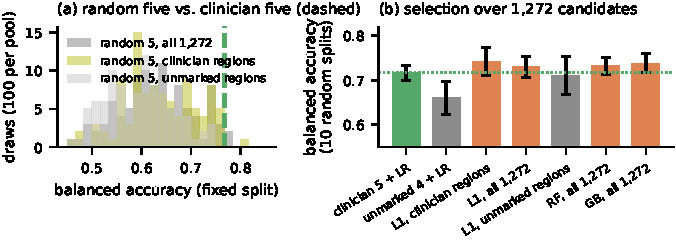
\includegraphics[width=0.95\linewidth]{figs/fig2_selection.pdf}
\caption{(a) Five measurements drawn at random from the bank (100 draws per pool; fixed
split) against the clinician-defined five. (b) Ten-partition mean $\pm$ s.d.\ of the five
against data-driven selection over the 1,272 candidates.}
\label{fig:selection}
\end{figure}

Fig.~\ref{fig:selection} asks whether \emph{any} five measurements would do. Five drawn at
random average $0.63$ (all regions), $0.64$ (clinician regions) and $0.60$ (unmarked
regions); the clinician-defined five sit at the 98th, 99th and 100th percentile of the 100
draws. Data-driven selection over all 1,272 candidates reaches $0.730\pm0.023$ ($\ell_1$),
$0.732\pm0.019$ (random forest) and $0.738\pm0.022$ (gradient boosting); restricting the
candidates to the clinician regions gives $0.742\pm0.032$ and to their complement
$0.710\pm0.043$ ($+0.03\pm0.05$, positive in 7/10 partitions): at the bank level the expert
boundary does not improve selection beyond noise. The honest reading is parsimony---five
named numbers equal the best of 1,272---and the annotation's value is in naming them.

\subsection{Evidence-gated fusion and ablations}

\begin{table}[t]
\centering
\caption{Ablations. Top: leave-one-out, region-group and single-quantity models (10
partitions). Bottom: fusion with the video branch under the same nested protocol, 9 groups.}
\label{tab:ablation}
\footnotesize
\setlength{\tabcolsep}{4pt}
\begin{tabular}{lcc}
\toprule
Measurement ablation (10 splits) & Balanced acc. & AUC \\
\midrule
all five & 0.717$\pm$0.017 & 0.787$\pm$0.016 \\
$-$ trunk lean & 0.682$\pm$0.017 & 0.767$\pm$0.016 \\
$-$ shoulder offset & 0.696$\pm$0.023 & 0.783$\pm$0.014 \\
$-$ head forward & 0.688$\pm$0.031 & 0.739$\pm$0.017 \\
$-$ max hip flexion & 0.723$\pm$0.020 & 0.790$\pm$0.015 \\
$-$ hip range & 0.731$\pm$0.010 & 0.800$\pm$0.010 \\
$-$ lumbar--pelvis group (3) & 0.713$\pm$0.019 & 0.793$\pm$0.012 \\
trunk lean alone & 0.707$\pm$0.011 & 0.778$\pm$0.009 \\
head forward alone & 0.409$\pm$0.070 & 0.399$\pm$0.069 \\
\midrule
Fusion (3 video branches $\times$ 3 seeds) & Balanced acc. & \\
\midrule
video branch alone & 0.628 & \\
5 quantities alone & 0.751 & \\
fixed $w{=}0.5$ / nested global $w$ / stacking & 0.717 / 0.745 / 0.731 & \\
sigmoid gate (6 features) & 0.773 & \\
\textbf{evidence gate} & 0.794 & \\
evidence gate, deviation permuted (10$\times$) & 0.743 & \\
evidence gate with TimeSformer video branch & 0.785 & \\
\bottomrule
\end{tabular}

\end{table}

\begin{figure}[t]
\centering
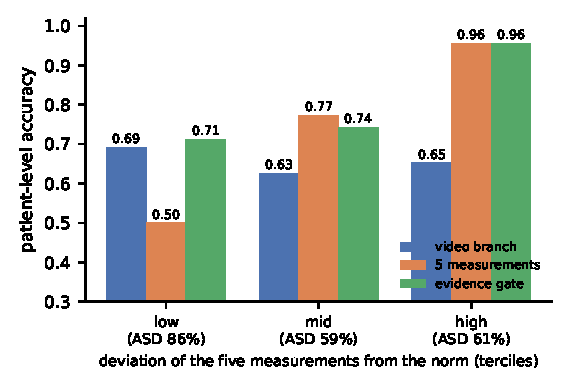
\includegraphics[width=0.46\linewidth]{figs/fig3_gate_strata.pdf}
\caption{Why the gate works: accuracy by tercile of $d$, pooled over the 9 fusion groups.
Where measurements are unremarkable (left; 86\% \asd) the five-number model is at chance
and the video model is not; where they deviate the five numbers are almost always right.}
\label{fig:strata}
\end{figure}

The video branch and the five numbers err on different patients: either being right would
give $0.90$. Table~\ref{tab:ablation} (bottom) shows what is recoverable honestly. A fixed
$w{=}0.5$ ($0.717$) and a nested global weight ($0.745$) do not beat the five numbers alone
($0.751$); stacking ($0.731$) and the sigmoid gate ($0.773$), whose coefficients collapse to
a near-constant weight, do little better. The evidence-strength gate reaches $0.794$
(grounded branch: $0.819$), non-negative against the five numbers in all nine groups and
against the nested weight in eight, and significant against the video branch in seven
(McNemar $p\le0.05$). The rule is stable: $\tau$ at the 30--40th percentile of $d$,
$w_{\mathrm{lo}}\in\{0,0.5\}$, $w_{\mathrm{hi}}=1$; any fixed $q\in[0.1,0.4]$ gives
$0.795$--$0.809$.

Fig.~\ref{fig:strata} shows the mechanism. In the tercile of least deviation 86\% of the
patients are \asd\ but the five-number model scores $0.50$: with normal-looking measurements
it defaults to non-\asd, and these are \asd\ patients without visible sagittal compensation,
whom the video model recognises at $0.69$; in the other terciles the five numbers are right
$0.77$ and $0.96$ of the time. Four controls close the argument: permuting $d$ across
patients drops the gate to $0.743$ (10 permutations per group; the true value exceeds all 30
permutations in a 79-patient run); computing $d$ from the four unmarked-region quantities
gives $0.733$, the permutation level; replacing the video branch by the TimeSformer gives
$0.785$; and leaving out head forward removes the gain entirely ($0.794\to0.729$, five-number
model at $0.740$), whereas leaving out any other quantity changes the gate by at most $0.03$.

The measurement ablation (Table~\ref{tab:ablation}, top) explains the last point.
\emph{Head forward alone} is uninformative ($0.41$; its direction even reverses because
dropped-head patients in the non-\asd\ group lean the head further), yet removing it costs
the most ($0.717\to0.688$, AUC $0.79\to0.74$). Head posture is a \emph{conditional} sign:
given the trunk inclination, the head's position relative to the trunk separates the
forward-inclined \asd\ patient from the dropped-head non-\asd\ patient. Trunk lean alone
gives $0.707$, and dropping the whole lumbar--pelvis group costs almost nothing ($0.713$)
because its three quantities are largely redundant: five numbers are, in effect, one strong
sign plus one conditional sign.

\subsection{Interpretability and negative results}

\begin{figure}[t]
\centering
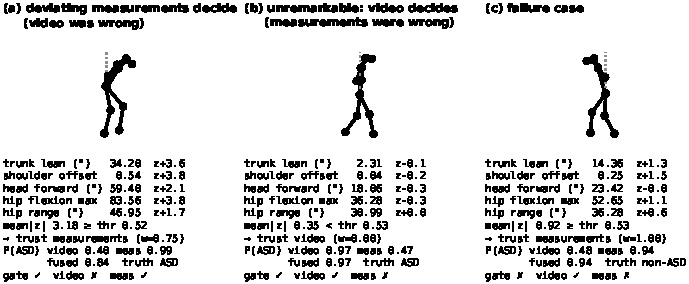
\includegraphics[width=\linewidth]{figs/fig4_explanations.pdf}
\caption{Readable decisions for three patients (grounded video branch, one seed): the five
quantities with $z$-scores, $d$ against the fold's threshold, the weight, and the branch and
fused probabilities.}
\label{fig:cards}
\end{figure}

The grounded branch keeps what the supervision bought: attention alignment $0.533\pm0.001$
(three seeds) against $0.135\pm0.034$ for Grad-CAM on the plain 3D CNN, $0.144$ for a
centre prior and $0.068$ for a uniform map; $0.104\pm0.012$ without the grounding loss and
$0.065$ when grounded to random locations; region presence AP $0.81$. The measurement
branch needs no such machinery: every decision is five numbers, their deviation, and which
branch was trusted (Fig.~\ref{fig:cards})---the classifier's input, not a post-hoc
rendering. Three negative lines bound the claims (supplement): feeding the five quantities
\emph{into} the video encoder, as auxiliary targets or by concatenation, never beats the
video baseline in 255 runs except one variant at $0.715\pm0.008$, still below the five
numbers alone; a soft region-weighted $\ell_1$ penalty on the bank is worse than a uniform
one; and five uses of a vision--language model (frozen features, zero-shot diagnosis at AUC
$0.44$, prompting, attribute questions, explanations) are at or below the 3D CNN. The gate
helps linear measurement branches but not the random forest or gradient boosting.

\section{Discussion, Limitations and Conclusion}

The same annotation helps as a prior and not as a signal because it is coarse as a label but
precise as a pointer: ``look at the trunk and the head'' translates into two well-defined
angles a linear model exploits, whereas a network given a saliency target learns where to
look without learning what the look means. That head posture is a conditional sign is, we
think, why clinicians mark the head; we flag it for clinical confirmation. The cohort is small (67 primary
patients, 21 non-\asd): intervals are about $\pm0.10$ wide and single-seed differences below
$0.08$ are noise, so every number here is a three-seed or ten-partition mean. Fusion is
evaluated on the fixed split only; the gate needs a linear, moderately accurate measurement
branch; monocular 3D gives no coronal-plane quantities; data come from one centre.

In conclusion, clinician attention is most useful not as something a gait network should
learn but as a specification of what to measure, and the evidence strength of those
measurements tells us when to trust them over the video.

\bibliographystyle{splncs04}
\bibliography{refs}

\end{document}
